\chapter{Giải pháp đề xuất}
Chúng tôi đã tiến hành xây dựng và thử nghiệm phương pháp phân đoạn lá gan trên các mô hình học sâu khác nhau.
\section{Mô hình 2D}
\section{Mô hình mạng nơ-ron tích chập 3D (CNN)}
\subsection{Chuẩn bị dữ liệu huấn luyện}
Phương pháp làm giàu giữ liệu:
\begin{itemize}
\item Thực hiện phép quay ngẫu nhiên từ -10 đến 10 độ quanh trục X.
\item Thực hiện phép quay ngẫu nhiên từ -10 đến 10 độ quanh trục Y.
\item Thực hiện phép quay ngẫu nhiên từ -45 đến 45 độ quanh trục Z.
\item Thực hiện phép biến đổi elastic với $\alpha = 1024$, $\alpha_{affine} = 40$, $\sigma = 40 $.
\item Cắt khối ngẫu nhiên với kích thước 192x192x64.
\end{itemize}
Dữ liệu từ các tập SLiver07 \cite{website:slvier07}, 3Dircadb \cite{website:data_3DIRCADb}, LiTS2017 \cite{website:LiTS} gồm 171 ảnh CT được chia làm hai phần 121 ảnh phần huấn luyện và 50 ảnh CT phần đánh giá :
\begin{itemize}
\item Phần huấn luyện (Training data): Đây là phần dùng để huấn luyện mô hình. Dữ liệu huấn luyện bao gồm 10080 mẫu dữ liệu với kích thước 192x192x64.
\item Phần đánh giá (Validation data): Đây là phần dùng để kiểm tra nếu mô hình quá khớp (Overfitting). Dữ liệu đánh giá bao gồm 1080 mẫu dữ liệu với kích thước 192x192x64.
\end{itemize}
\subsection{Xây dựng mô hình mạng nơ-ron tích chập 3 chiều}
Dựa trên kiến trúc mạng nơ-ron tích chập 3 chiều và phương pháp huấn luyện giám sát sâu\cite{dsn_paper} của Qi Dou và cộng sự, chúng tôi đã xây dựng mô hình phù hợp và có thể huấn luyện trên máy ảo google colab (Hình \ref{our_CNN_org}). Mô hình này gồm hai phần: phần mã hóa và phần giải mã. Trong phần mã hóa, chúng tôi đã sử dụng bốn lớp Max pooling với stride 2x2x2 và các lớp tích chập với activation ELU. Sau phần mã hóa, kích thước bản đồ đặc trưng đã giảm kích thước đầu vào 192x192x64x1 còn 12x12x4x256. Phần giải mã chỉ sử dụng bốn lớp đảo tích chập với stride 2x2x2 và một lớp sigmoid. Đầu ra của lớp Sigmoid là một bản đồ xác xuất có kích thước 192x192x64x1. Mỗi giá trị trong bản đồ xác xuất này là xác xuất mà voxel tương ứng ở đầu vào là gan.

\begin{figure}[h]
\centering
    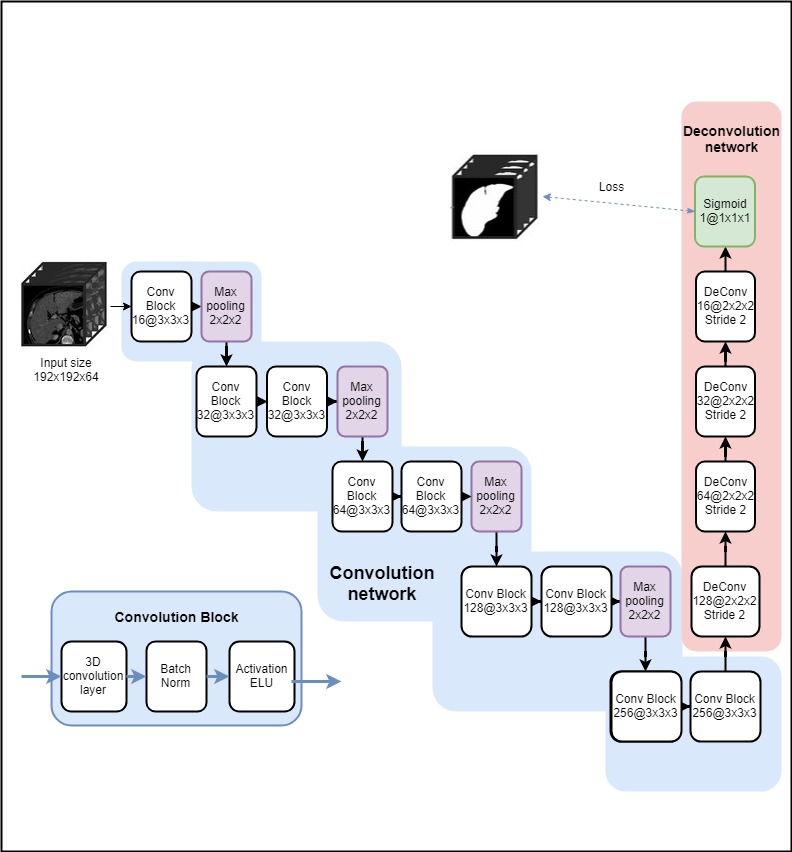
\includegraphics[totalheight=15cm]{Images/CNN_org.jpg}
    \caption{Kiến trúc mạng nơ-ron tích chập 3-chiều đề xuất}
    \label{our_CNN_org}
\end{figure}
\subsection{Huấn luyện mạng và kết quả thực nghiệm}
\paragraph{Phương pháp huấn luyện giám sát sâu:}
Mạng nơ-ron tích chập 3D được biến đổi và huấn luyện theo phương pháp giám sát sâu. Theo phương pháp này, chúng tôi đã thêm một số phần giải mã (decoder) thích hợp vào mạng nơ-ron như Hình \ref{our_CNN}. Hàm mất mát (loss function) sẽ được tính từ hàm mất mát của tất cả các phần giải mã:\\
\begin{center} $Loss = \mu_1 Loss_{aux1} + \mu_2 Loss_{aux2}+\mu_3 Loss_{aux3}+\mu_4 Loss_{main}$\end{center}
\begin{figure}[h]
\centering
    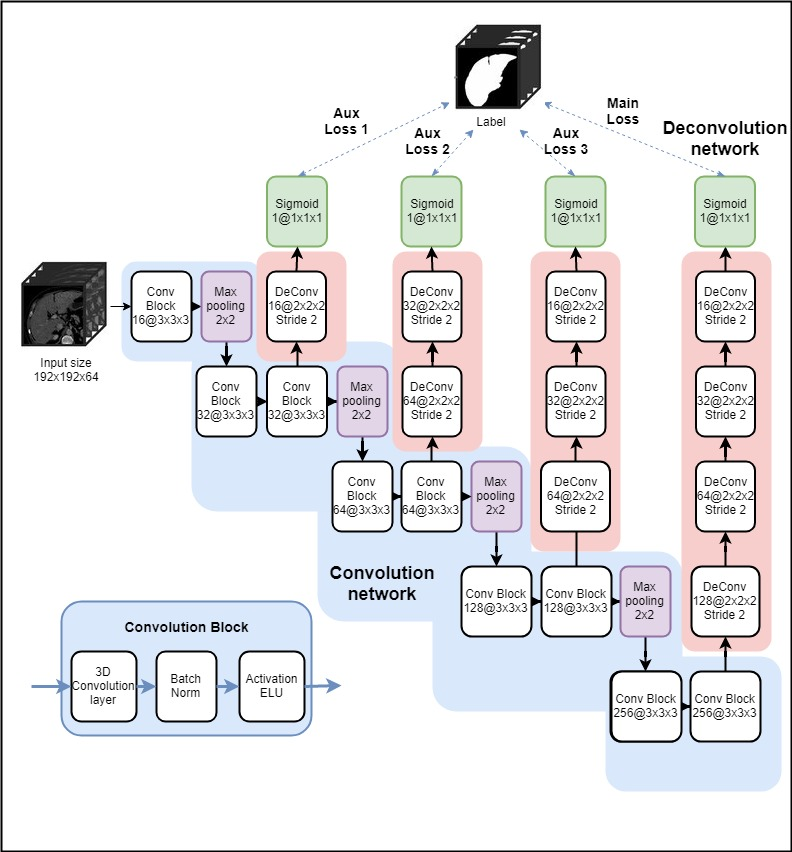
\includegraphics[totalheight=15cm]{Images/CNN.jpg}
    \caption{Kiến trúc mạng nơ-ron tích chập 3-chiều giám sát sâu đề xuất. Ba phần giải mã phụ được thêm vào trước lớp Max pooling.}
    \label{our_CNN}
\end{figure}
\paragraph{Thông số huấn luyện mô hình}
\begin{itemize}
\item Máy tính sử dụng: Máy ảo Google Colab với card đồ họa GPU Tesla T4.
\item Framework: Tensorflow 1.13.1.
\item Ngôn ngữ: Python 3.6.4.
\item Hàm mất mát (Loss function): Cross entropy loss.
\item Phương pháp tối ưu: Adam optimizer.
\item Các siêu tham số: Learning rate 0.0001, L2 regularization 0.0001.
\item Các tham số tổng hợp hàm mất mát: $\mu_1 = 1$,  $\mu_2 = 2$,  $\mu_3 = 4$,  $\mu_4 = 8$
\end{itemize}
\paragraph{Kết quả}
Mô hình CNN được đánh giá trên các hệ thống đánh giá kết quả tự động mang tính khách quan cao trên tập kiểm thử SLIVER07 và LITS2017 (Bảng \ref{tab:CNN-SLIVER07_Test}). Ngoài ra chúng tôi đã tự đánh giá mô hình này trên tập dữ liệu 3Dircadb batch 1. Phương pháp này đã đạt kết quả khá tốt trên tập SLIVER07 và 3Dircadb với độ đo VOE thấp hơn 6\%. Đây là một kết quả có thể chấp nhận được và sử dụng cho việc xây dựng mô hình lá gan. Tuy nhiên, khả năng hân đoạn của mô hình CNN còn khá hạn chế trên tập kiểm thử LiTS2017.
\begin{table}[]
\begin{tabular}{|c|c|c|c|c|}
\hline
\textbf{Độ Đo} & \textbf{SLIVER07 (train)} & \textbf{SLIVER07 (test)} & \textbf{3Dircadb\_b1} & \textbf{LiTS2017 (test)} \\ \hline
VOE            & 3.72                      & 5.58                     & 4.69                  & 8.80                     \\ \hline
RVD            & 0.13                      & -0.19                    & -0.26                 & 2.60                     \\ \hline
AvgD           & 0.49                      & 0.86                     & 0.59                  & 1.44                     \\ \hline
RMSD           & 1.03                      & 1.77                     & 1.21                  & 2.82                     \\ \hline
MaxD           & 14.00                     & 20.79                    & 17.41                 & 24.94                    \\ \hline
Score          & 87.54                     & 79.89                    & 83.98                 & \_                       \\ \hline
Dice per case  & 98.10                     & \_                       & 97.60                 & 95.3                     \\ \hline
Dice global    & \_                        & \_                       & \_                    & 95.8                     \\ \hline
\end{tabular}
\caption{\label{tab:CNN-SLIVER07_Test}Kết quả đánh giá mô hình CNN trên ba tập dữ liệu SLIVER07, 3Dircadb và LiTS2017.}
\end{table}

\section{Mô hình Unet 3D}
\subsection{Phương pháp Tranfer Learning cho bài toán phân đoạn ảnh}
Tranfer learning hay Fine-tuning là phương pháp sử dụng lại trọng số của một số lớp, hoặc toàn bộ các lớp của một mô hình đã được huấn luyện trước đó để khởi tạo cho các lớp trên mô hình mới. Mô hình mới sẽ được huấn luyên với dữ liệu khác có tính tương quan cao hoặc khác hoàn toàn với nguồn dữ liệu cũ.
Phương pháp huấn luyện với mô hình mới phụ thuộc vào độ tương quan giữa dữ liệu cũ và dữ liệu mới và kích thước của dữ liệu mới:
\begin{itemize}
\item Dữ liệu mới là nhỏ hơn và tương tự như dữ liệu gốc: vì dữ liệu mới nhỏ và có độ tương quan cao với dữ liệu cũ nên việc huấn luyện lại mô hình dễ dẫn đến hiện tượng quá khớp (overfitting). Vì vậy, chỉ huấn luyện lại phần giãi mã dựa trên đặc trưng thu được qua phần mã hóa gốc.
\item Dữ liệu mới là lớn và tương tự như dữ liệu gốc: vì dữ liệu mới lớn, hiện tượng quá khớp (overfitting) khó có khả năng xảy ra nên có thể huấn luyện toàn bộ mô hình với learning rate nhỏ.
\item Dữ liệu mới là nhỏ và rất khác so với dữ liệu gốc: sử dụng bộ giải mã đơn giản và chỉ huấn luyện một số lớp cuối cùng.
\item Dữ liệu mới là lớn và rất khác so với dữ liệu gốc: có thể khởi tạo từ bộ trọng số cũ, không cần phải huấn luyện lại từ đầu.
\paragraph{Dữ liệu huấn luyện Unet 3-chiều} Chúng tôi tạo ra ba bộ dữ liệu riêng biệt từ mỗi tập SLIVER07, 3Dircadb và LiTS2017 với phương pháp làm giàu như dữ liệu huấn luyện mô hình CNN. Mỗi bộ dữ liệu mới này sẽ nhỏ hơn rất nhiều so với dữ liệu huấn luyện mô hình CNN (~2000 mẫu/1 bộ so với 10080 mẫu dữ liệu cũ).
\paragraph{Sử dụng phương pháp Tranfer Learning trên mô hình Unet 3-chiều} Chúng tôi đã sử dụng lại toàn bộ phần mã của mô hình CNN cho mô hình Unet 3-chiều. Chúng tôi chỉ thực hiện huấn luyện phần giải mã và nối tắt với mỗi bộ dữ liệu.
\end{itemize}
\subsection{Xây dựng mô hình mạng Unet 3-chiều}
Mô hình Unet 3-chiều này được xây dựng dựa trên cơ sở mô hình Unet 3-chiều \cite{3DUnet} của Ozgun Cikek và cộng sự và một số thay đổi ở cả ba phần giải mã, mã hóa và nối tắt. (Hình \ref{Unet3D_pro})
\paragraph{Phần mã hóa} Phần mã hóa của mô hình Unet 3-chiều này sử dụng lại kiến trúc và trọng số phần mã hóa của mô hình tích chập 3 chiều (CNN) mà chúng tôi đã đề cập ở phần trước.
\paragraph{Phần nối tắt} Chúng tôi đã thêm một lớp tích chập với kích thước cửa sổ 5x5 vào phần nối tắt để giảm số kênh (channel) trước khi kết hợp với kết quả lớp đảo tích chập tương ứng.
\paragraph{Phần giải mã} Phần giải mã được chỉnh sửa số cửa sổ trên các lớp tích chập, đảo tích chập dể phù hợp với phần mã hóa.
\begin{figure}[h]
\centering
    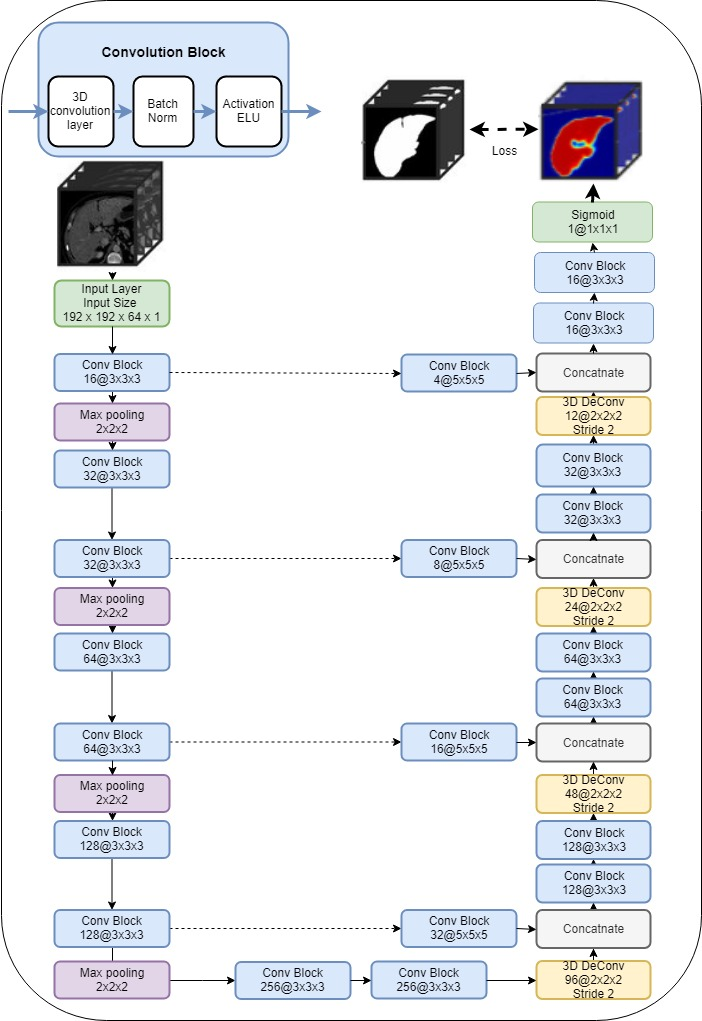
\includegraphics[totalheight=23cm]{Images/UNET3D_pro.jpg}
    \caption{Kiến trúc mô hình Unet 3-chiều đề xuất}
    \label{Unet3D_pro}
\end{figure}
\subsection{Huấn luyện mạng và kết quả}
\paragraph{Thông số huấn luyện mô hình}
\begin{itemize}
\item Máy tính sử dụng: Máy ảo Google Colab với card đồ họa GPU Tesla T4.
\item Framework: Tensorflow 1.13.1.
\item Ngôn ngữ: Python 3.6.4.
\item Hàm mất mát (Loss function): Cross entropy loss.
\item Phương pháp tối ưu: Adam optimizer.
\item Các siêu tham số: Learning rate 0.0001.
\end{itemize}
\paragraph{Kết quả}
Chúng tôi thực hiện đánh giá mô hình Unet 3-chiều trên tập dữ liệu tương ứng đã sử dụng khi huấn luyện (Ví dụ: Nếu huấn luyện mô hình với dữ liệu được làm giàu từ tập LITS2017 thì sẽ đánh giá trên tập kiểm thử của tập này). Mô hình Unet 3-chiều đã đạt kết quả rất tốt trên cả ba tập SLIVER07 (tập huấn luyện), 3Dircadb batch 1 và LiTS2017 (tập kiểm thử).
\begin{table}[]
\begin{tabular}{|c|c|c|c|}
\hline
\textbf{Độ Đo} & \textbf{SLIVER07 (train)} & \textbf{3Dircadb\_b1} & \textbf{LiTS2017 (test)} \\ \hline
VOE            & 2.67                      & 2.57                  & 7.60                     \\ \hline
RVD            & 0.39                      & -0.14                 & 0.02                     \\ \hline
AvgD           & 0.32                      & 0.26                  & 1.20                     \\ \hline
RMSD           & 0.65                      & 0.55                  & 2.54                     \\ \hline
MaxD           & 8.26                      & 7.82                  & 23.92                    \\ \hline
Score          & 91.81                     & 92.61                 & \_                       \\ \hline
Dice per case  & 98.65                     & 98.69                 & 96.00                    \\ \hline
Dice global    & \_                        & \_                    & 96.60                     \\ \hline
\end{tabular}
\caption{\label{tab:CNN-SLIVER07_Test}Kết quả đánh giá mô hình UNET3D trên ba tập dữ liệu SLIVER07, 3Dircadb và LiTS2017.}
\end{table}



